
\chapter{PLANOS Y LÁMINAS DE DETALLE}

\begin{longtable}{L{1.6cm}L{5.5cm}L{4.5cm}L{2cm}}
	\caption{Relación de planos presentados}
	\label{tab:planos}\\
	
	\toprule
	\textbf{Código} & \textbf{Descripción} & \textbf{Archivo} & \textbf{Estado} \\
	\midrule
	\endfirsthead
	
	\toprule
	\textbf{Código} & \textbf{Descripción} & \textbf{Archivo} & \textbf{Estado} \\
	\midrule
	\endhead
	
	IE-01 &
	Plano de Instalaciones Eléctricas - Primer Piso &
	plano\_electrico\_piso\_1.png &
	Entregado \\
	
	IE-02 &
	Plano de Instalaciones Eléctricas - Segundo Piso &
	plano\_electrico\_piso\_2.png &
	Entregado \\
	
	IE-03 &
	Plano de Instalaciones Eléctricas - Tercer Piso &
	plano\_electrico\_piso\_3.png &
	Entregado \\
	
	IE-04 &
	Plano de Recorrido de Canalizaciones (Detalles en Planta) &
	plano\_electrico\_piso\_1/2/3.png &
	Entregado \\
	
	IE-05 &
	Diagrama Unifilar y Cuadro de Cargas &
	diagrama\_unifilar.pdf &
	Entregado \\
	
	IE-06 &
	Detalle del Sistema de Puesta a Tierra &
	puesta\_a\_tierra.pdf &
	Entregado \\
	
	\bottomrule
\end{longtable}

\section{Planos de Instalaciones Eléctricas}

Los planos mostrados a continuación presentan la distribución de luminarias, interruptores, tomacorrientes y canalizaciones eléctricas correspondientes a cada nivel de la vivienda unifamiliar. Asimismo, se indica el recorrido de los circuitos derivados y la ubicación de los diferentes elementos de la instalación eléctrica proyectada.

\subsection{IE-01: Plano de Instalaciones Eléctricas – Primer Piso}

Se presenta el plano correspondiente al primer nivel de la vivienda, donde se muestra la distribución de los puntos de alumbrado, tomacorrientes, interruptores y canalizaciones eléctricas.

\begin{figure}[H]
	\centering
	
\includegraphics[
	width=\textwidth,
	height=0.76\textheight,
	keepaspectratio
	]{06_planos/entregables/png/plano_electrico_piso_1.png}
	\caption{Plano de Instalaciones Eléctricas - Primer Piso}
	\label{fig:piso1}
\end{figure}

\subsection{IE-02: Plano de Instalaciones Eléctricas – Segundo Piso}

Se presenta el plano correspondiente al segundo nivel de la vivienda, donde se muestra la distribución de los puntos de alumbrado, tomacorrientes, interruptores y canalizaciones eléctricas.

\begin{figure}[H]
	\centering
	
\includegraphics[
	width=\textwidth,
	height=0.76\textheight,
	keepaspectratio
	]{06_planos/entregables/png/plano_electrico_piso_2.png}
	\caption{Plano de Instalaciones Eléctricas - Segundo Piso}
	\label{fig:piso2}
\end{figure}

\subsection{IE-03: Plano de Instalaciones Eléctricas – Tercer Piso}

Se presenta el plano correspondiente al tercer nivel de la vivienda, donde se muestra la distribución de los puntos de alumbrado, tomacorrientes, interruptores y canalizaciones eléctricas.

\begin{figure}[H]
	\centering
	
\includegraphics[
	width=\textwidth,
	height=0.76\textheight,
	keepaspectratio
	]{06_planos/entregables/png/plano_electrico_piso_3.png}
	\caption{Plano de Instalaciones Eléctricas - Tercer Piso}
	\label{fig:piso3}
\end{figure}

\subsection{IE-05: Diagrama Unifilar y Cuadro de Cargas}

Se presenta el diagrama unifilar correspondiente a los circuitos derivados, tableros de distribución y sistema de puesta a tierra.

\begin{landscape}
	\begin{figure}[H]
		\centering
		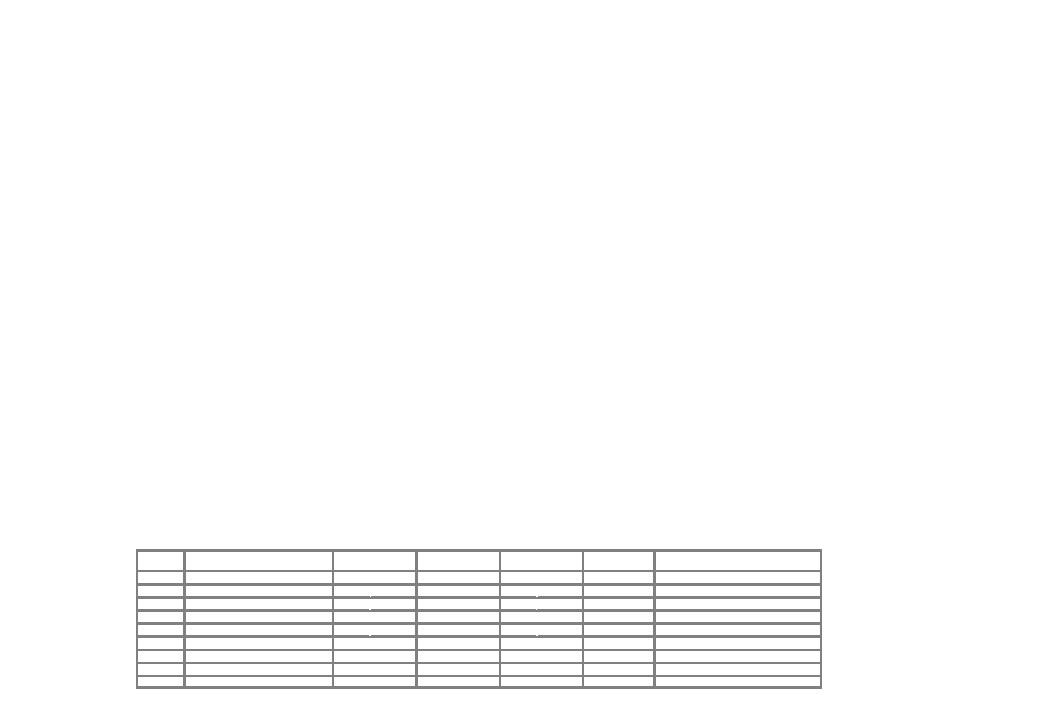
\includegraphics[
		width=\textwidth,
		height=0.82\textheight,
		keepaspectratio
		]{06_planos/diagramas/diagrama_unifilar.pdf}
		\caption{Diagrama Unifilar - Tablero General TG-01}
		\label{fig:unifilar}
	\end{figure}
\end{landscape}

\subsection{IE-06: Detalle del Sistema de Puesta a Tierra}

Se presenta la lámina de detalle correspondiente a la instalación del sistema de puesta a tierra (pozo a tierra).

\begin{landscape}
	\begin{figure}[H]
		\centering
		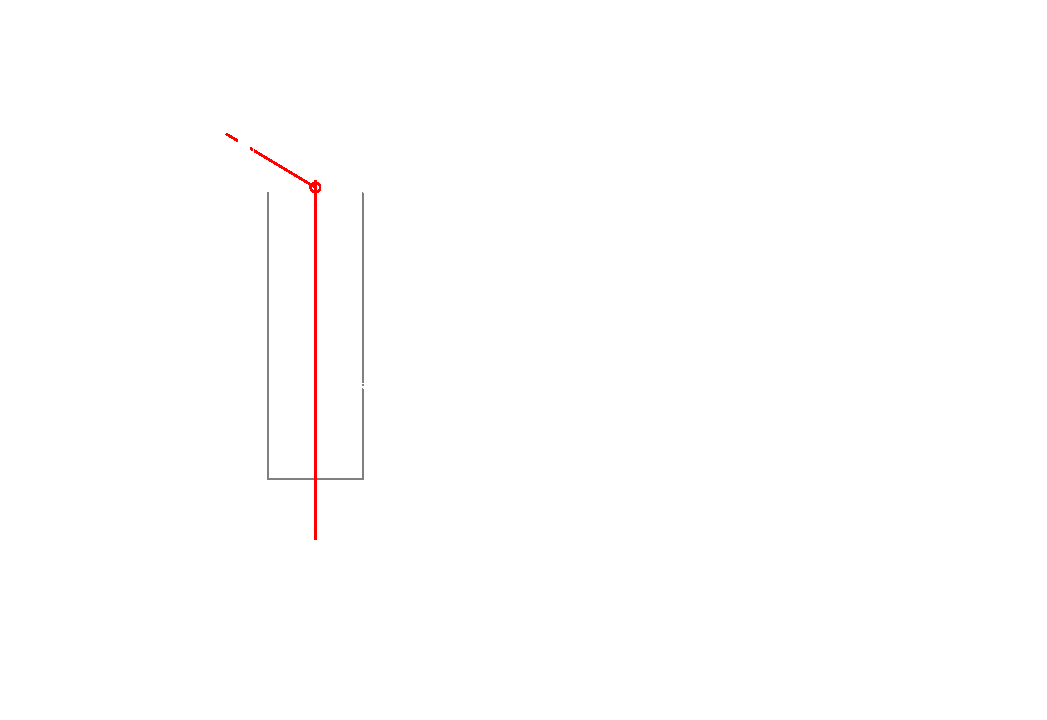
\includegraphics[
		width=\textwidth,
		height=0.82\textheight,
		keepaspectratio
		]{06_planos/diagramas/puesta_a_tierra.pdf}
		\caption{Plano de Detalle del Sistema de Puesta a Tierra}
		\label{fig:puesta_tierra}
	\end{figure}
\end{landscape}

\section{Observaciones}

\begin{itemize}
	\item Los planos fueron elaborados considerando la distribución arquitectónica de la vivienda unifamiliar de tres niveles.
	
	\item La ubicación de luminarias, interruptores y tomacorrientes se realizó de acuerdo con los criterios de funcionalidad y seguridad establecidos en el diseño eléctrico residencial.
	
	\item Las canalizaciones eléctricas fueron trazadas procurando recorridos técnicamente adecuados y compatibles con la distribución de los ambientes.
	
	\item El diseño fue desarrollado considerando los criterios establecidos en el Código Nacional de Electricidad -- Utilización (CNE-U).
\end{itemize}
